\documentclass[10pt]{article}
\usepackage{amsmath, amssymb}
\usepackage{geometry}
\usepackage{booktabs}
\usepackage{caption}
\usepackage{graphicx}
\usepackage{hyperref}
\usepackage[utf8]{inputenc}
\usepackage{lmodern}
\usepackage{float}
\usepackage{tikz}
\usetikzlibrary{arrows.meta, calc}

\geometry{margin=1in}

\title{A Mathematical Gem: The Hyperbolic Boundary is Not at Infinity --- It's a Relativistic Shadow}
\author{Steven Klemmer\\
\small Independent Researcher\\
\small \texttt{stevenklemmer@icloud.com}\\
\small \url{https://github.com/stevenk42}}
\date{\today}

\begin{document}

\maketitle

\begin{abstract}
Students of hyperbolic geometry are told that geodesics reach the ``ideal boundary'' in finite time --- yet distances to that boundary are infinite, and dynamics appear to freeze. This paradox has no resolution within the disk or half-plane models alone. But lift your gaze: embed $\mathbb{H}^2$ into Minkowski space, and the mystery dissolves. The boundary is not a spatial infinity --- it is the \emph{projection} of light-like geodesics. Time dilation and length contraction from special relativity explain why clocks halt and shapes flatten as objects approach $|z|=1$. Though implicit in the hyperboloid model, this interpretation is absent from nearly all textbooks --- leaving generations of learners confused. Here, we restore the missing link between geometry and physics, turning paradox into clarity.
\end{abstract}

\section*{Introduction: The Frozen Edge of the Disk}

Open any textbook on hyperbolic geometry. You'll find the Poincaré disk, its geodesics curving gracefully toward the unit circle, and a footnote: ``The boundary consists of ideal points at infinity.'' Then comes the cognitive dissonance:

\begin{itemize}
    \item A particle following a radial geodesic reaches $|z| = 1$ in finite proper time.
    \item Yet the hyperbolic distance to the boundary is infinite.
    \item Internal dynamics --- rotation, vibration, ticking clocks --- appear to freeze as the boundary is approached.
\end{itemize}

Zeno would be proud. How can something arrive in finite time if it must traverse infinite distance? Why do clocks stop? Why does the boundary feel more like an event horizon than a geometric edge?

The standard answer --- ``It's just how the metric behaves'' --- is mathematically correct but intellectually unsatisfying. What's missing is not rigor, but \emph{physical intuition}. And that intuition lies not in two dimensions, but in three --- with a dash of Einstein.

\begin{figure}[H]
\centering
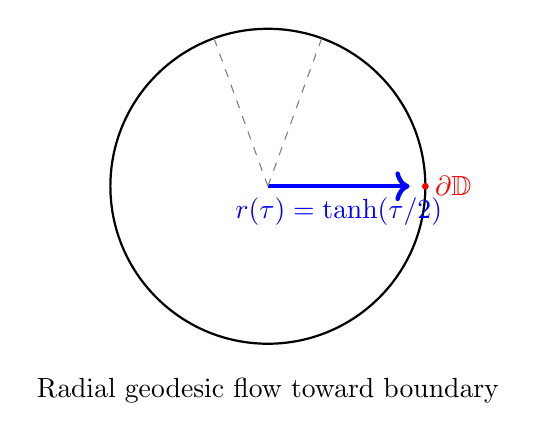
\begin{tikzpicture}[scale=2]
    \draw[thick] (0,0) circle (1);
    \draw[->, blue, ultra thick] (0,0) -- (0.9,0) node[midway, below] {$r(\tau) = \tanh(\tau/2)$};
    \filldraw[red] (1,0) circle (0.5pt) node[right] {$\partial\mathbb{D}$};
    \draw[gray, dashed] (0,0) -- (70:1);
    \draw[gray, dashed] (0,0) -- (110:1);
    \node at (0,-1.3) {Radial geodesic flow toward boundary};
\end{tikzpicture}
\caption{Proper time $\tau$ drives $r \to 1$. Dynamics freeze not from failure --- but from projection.}
\label{fig:radial_flow}
\end{figure}

\section*{The Hidden Stage: Minkowski Space}

The key is the \textbf{hyperboloid model}: the surface $X^2 + Y^2 - T^2 = -1$, $T > 0$, embedded in $(2+1)$-dimensional Minkowski space with metric $ds^2 = dX^2 + dY^2 - dT^2$. This is not just an alternative model --- it's the \emph{mother space} from which all others descend by projection.

In this space, a radial geodesic looks like:
\begin{equation*}
\Gamma(\tau) = (0, \sinh\tau, \cosh\tau).
\end{equation*}
Its proper time is simply $\tau$, and as $\tau \to \infty$, it asymptotically approaches the light ray $(0, s, s)$ --- never intersecting it, always remaining timelike. No infinity is reached; no incompleteness arises. The geodesic is blissfully complete.

Now project this path onto the Poincaré disk via the standard map:
\begin{equation*}
z = \frac{X + iY}{T + 1} \implies z(\tau) = i \cdot \frac{\sinh\tau}{\cosh\tau + 1} = i \cdot \tanh(\tau/2).
\end{equation*}
As $\tau \to \infty$, $|z| \to 1$. But here's the catch: the Poincaré metric,
\begin{equation*}
ds_P = \frac{2\,|dz|}{1 - |z|^2},
\end{equation*}
blows up near the boundary --- not because anything is singular in the geometry, but because the \emph{projection stretches null asymptotics into infinite coordinate distance}.

\begin{figure}[H]
\centering
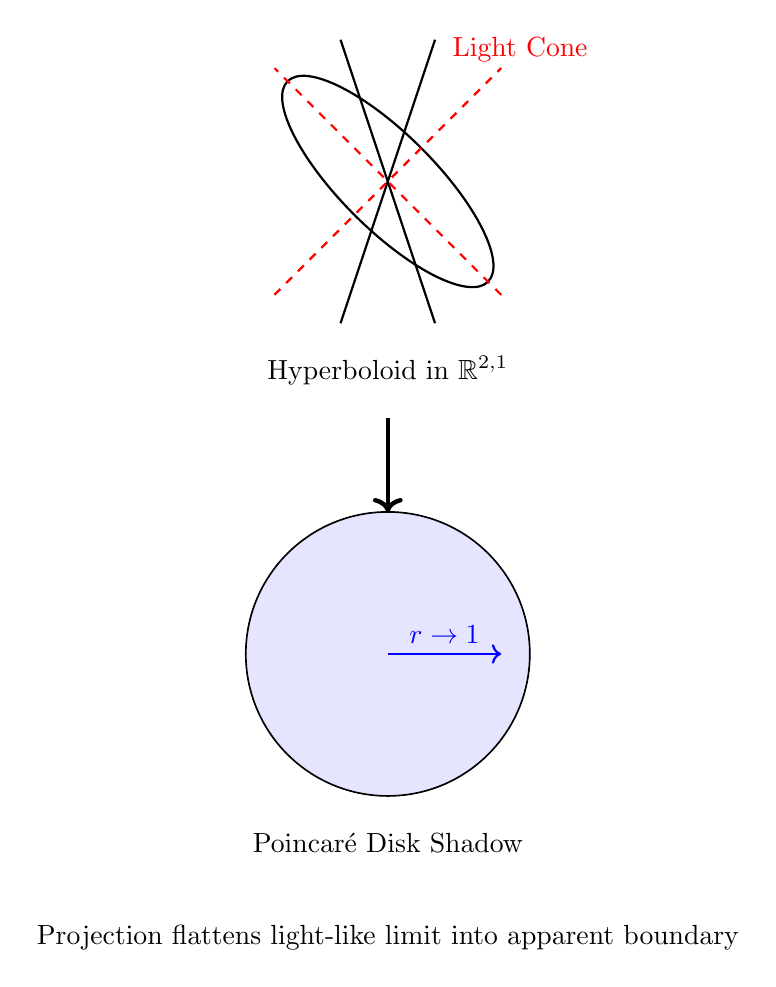
\begin{tikzpicture}[scale=1.2]
% Draw hyperboloid sheet (simplified)
\draw[thick, rotate around={45:(0,0)}] (0,0) ellipse (0.5 and 1.5);
\draw[thick] (-0.5,-1.5) -- (0.5,1.5);
\draw[thick] (0.5,-1.5) -- (-0.5,1.5);

% Light cone (asymptotes)
\draw[dashed, red, thick] (-1.2,-1.2) -- (1.2,1.2);
\draw[dashed, red, thick] (1.2,-1.2) -- (-1.2,1.2);

% Label
\node at (0,-2) {Hyperboloid in $\mathbb{R}^{2,1}$};
\node[red] at (1.4,1.4) {Light Cone};

% Arrow down
\draw[->, ultra thick] (0,-2.5) -- (0,-3.5);

% Poincare Disk below
\draw[thick] (0,-5) circle (1.5);
\draw[fill=blue!10] (0,-5) circle (1.5);
\draw[->, blue, thick] (0,-5) -- (1.2,-5) node[midway, above] {$r \to 1$};
\node at (0,-7) {Poincar\'e Disk Shadow};

% Annotation
\node[align=center] at (0,-8) {Projection flattens light-like limit into apparent boundary};
\end{tikzpicture}
\caption{The hyperboloid (top) projects to the Poincaré disk (bottom). The light cone (red) maps to the disk boundary $|z| = 1$, where dynamics appear to freeze.}
\label{fig:projection}
\end{figure}

\section*{Relativity Enters the Geometry Classroom}

Why do clocks slow down near the boundary? Why do objects flatten?

Because in the embedding space, the geodesic is becoming \emph{asymptotically light-like} --- and we know from special relativity what happens then:

\begin{itemize}
\item \textbf{Time dilation}: As velocity $\to c$, proper time slows relative to lab frame.
\item \textbf{Length contraction}: Objects contract along direction of motion.
\end{itemize}

These effects survive projection:

\begin{itemize}
\item The ``freezing clock'' is projected time dilation.
\item The ``flattened shape'' is projected length contraction.
\end{itemize}

The boundary isn't a place --- it's a \emph{limit state}, where worldlines become null, and their temporal evolution vanishes from the projected view. What we call ``the boundary'' is just the shadow cast by light rays on the screen of our 2D model.
\\
\\
\section*{One Point, Many Paths: The Bidirectionality Mystery}

Another oddity: multiple geodesics can ``end'' at the same boundary point. Worse, boundary points seem to encode directional information --- they're labeled by angles, not locations.

Resolution? Each boundary point corresponds not to a point, but to an entire \emph{null ray} on the future light cone. Consider two geodesics:
\begin{equation*}
\Gamma_1(\tau) = (\sinh\tau, 0, \cosh\tau), \quad \Gamma_2(\tau) = (0, \sinh\tau, \cosh\tau).
\end{equation*}
Their projections go to $z=1$ and $z=i$. But infinitesimally perturb $\Gamma_1$ toward $\Gamma_2$, and the endpoint moves smoothly along the circle. The boundary point $z=1$ thus encodes not a location, but a \emph{direction of approach} --- an equivalence class of geodesics asymptoting to the null ray $(s, 0, s)$.

The boundary is not a set of points. It's a catalog of light-like futures.

\section*{Why Hasn't This Been Taught?}

Good question.

The hyperboloid model appears in advanced texts (Thurston, Ratcliffe, Cannon), and its connection to Minkowski space is well known to geometers and relativists. But the \emph{pedagogical leap} --- using SR to explain boundary behavior --- is almost never made explicit.

Why? Perhaps because:

\begin{itemize}
\item Geometers avoid physics metaphors.
\item Physicists rarely teach pure hyperbolic geometry.
\item Textbooks prioritize formalism over intuition.
\end{itemize}

The result? Students memorize ``ideal points at infinity'' without ever understanding \emph{why} the boundary behaves so strangely.

We can do better.

\section*{Conclusion: A Bridge Between Worlds}

This reinterpretation requires no new mathematics --- only a shift in perspective. By viewing the hyperbolic plane as a spacelike slice of Minkowski space, and its boundary as the celestial sphere of light rays, we replace abstract infinity with concrete physics.

The freezing of clocks? Time dilation.
The flattening of shapes? Length contraction.
The multiplicity of paths to one point? Null ray equivalence.
The existence of multiple models? Different camera angles on the same object.

None of this is technically new. But as a \emph{teaching framework}, it is revolutionary. It turns confusion into clarity, paradox into prediction, and dread into delight.

Next time you see the Poincaré disk, don't look at the boundary as a wall --- look through it, into the higher-dimensional spacetime casting its shadow. The ``ideal points'' were never at infinity. They were light rays all along.

\section*{Acknowledgments}

The author thanks coffee, curiosity, and the silent army of students who stared at the unit circle wondering, ``Why does time stop here?''

\section*{Conflict of Interest}
The author declares no conflicts of interest.

\section*{Funding}
This research received no external funding.

\appendix

\section*{Appendix: Metric Degeneracy at the Light Cone}

On the light cone $X^2 + Y^2 = T^2$, the induced metric from Minkowski space degenerates:
\begin{equation*}
ds_{\text{induced}}^2 = dX^2 + dY^2 - dT^2 = 0 \quad \text{(along generators)},
\end{equation*}
reflecting the loss of a timelike direction. Transverse displacements (e.g., changing angle) remain spacelike, preserving a 1D spatial metric on the celestial sphere --- consistent with the angular labeling of the boundary in the disk model.

\end{document}
